\documentclass[11pt, oneside]{article}
\usepackage[margin=1in,letterpaper]{geometry}
\usepackage{times}
\usepackage{graphicx}
\usepackage{amssymb,amsmath,mathtools}
\usepackage{array}
\usepackage{longtable}
\usepackage{color}
\usepackage[T1]{fontenc}
\usepackage{sectsty}
\usepackage{tikz}
\usetikzlibrary{decorations.markings,calc,patterns,arrows.meta}
\usepackage{pgfplots}
\pgfplotsset{compat=1.17}
\sectionfont{\fontsize{12}{12}\selectfont}
\subsectionfont{\fontsize{11}{11}\selectfont}
\subsubsectionfont{\normalsize\itshape\mdseries}

\renewcommand\labelitemi{{\boldmath$\cdot$}}

%%%%%%%%%%%%%%%%%%%%%%%%%%%%%%%%%%%%%
% Notation: symbols follow ../variables_master.tex. Renames that apply existing instructor decisions (each also marked
% at first use):
%   - power densities S -> script \mathcal{S} (D10): S_0^i, S_q^i(z), S_p^s (-> \mathcal{S}_{r,p}, D81);
%   - distance to the antenna r -> R (D53);
%   - EM wavenumber K_0 -> k_0 (D14);
%   - air-snow transmissivities T_p, T_q -> \mathbb{T}_p, \mathbb{T}_q (D19: T is temperature only);
%   - reflectivities Gamma^p, Gamma^p_coh (polarization as a superscript, as in Ulaby & Long) -> Gamma_p, Gamma_p^coh
%     (polarization as a subscript, as for Gamma_h, Gamma_v in the master table, L5).
% Instructor decisions (2026-09-29, master table D76--D84): renamed (resolved): handwritten sigma-hat_v^back,
% sigma-hat_v^bist -> sigma-hat^back_pq, sigma-hat^bist_pq (D76, subscript v dropped); handwritten angles
% theta_i' = theta_s' (= pi/2 - theta_i) written as pi/2 - theta_i explicitly (D78); coherent-addition factor
% c -> c_add (D79); scattered power density S_p^s -> \mathcal{S}_{r,p} (as S_r in L7, D81). Kept (approved): N_v (D77),
% "transmissivity" for Upsilon (canopy) and \mathbb{T} (interface) (D80), kappa_e, kappa_a, kappa_s and sigma^0_s (D81),
% subscript 0 in A_0, S_0^i (D82), Gamma_p (D83), delta_p (D84).
% Descriptive subscripts (e, a, s, v, g, c, coh, back, bist, rer, veg) are upright, as in Ulaby & Long; the
% polarization indices p, q are italic.
% Main reference checks: Ulaby & Long (2014), Secs. 11-1 to 11-4 (pp. 461-469), Eq. 5.110 (p. 199), Eqs. 11.51,
% 11.55 (pp. 474-475); Liou (2002), Eq. 3.3.7 (p. 89).
%%%%%%%%%%%%%%%%%%%%%%%%%%%%%%%%%%%%%

\newcommand{\ke}[1]{\kappa_\mathrm{e}^{#1}}
\newcommand{\sback}{\hat{\sigma}^\mathrm{back}_{pq}}
\newcommand{\sbist}{\hat{\sigma}^\mathrm{bist}_{pq}}
\newcommand{\Gc}[1]{\Gamma_{#1}^\mathrm{coh}}

\title{Ge158 Lecture 9: Volume Scattering}
\author{Brent Minchew}
\date{}

\setlength{\emergencystretch}{1.5em}
\begin{document}
\maketitle

\noindent\underline{\textbf{Topics covered}}
\begin{itemize}
	\item Fundamentals of volume scattering
	\item Heuristic scattering from vegetation
	\item Heuristic scattering from snow
\end{itemize}

%%%%%%%%%%%%%%%%%%%%%%%%%%%%%%%%%%%%%
\section{Basics of volume scattering from heterogeneous media}
\label{s:basics}

\begin{itemize}
	\item Distinction between surface and volume scattering
	\begin{itemize}
		\item Surface scattering
		\begin{itemize}
			\item Reflectivity a function of
			\begin{enumerate}
				\item dielectric constant of surface;
				\item tilting of surface relative to plane of incidence (i.e., long-wavelength ($\gg\lambda$) surface height variations).
			\end{enumerate}
			% NOTE: kept as handwritten (with its underline). The roughness spectrum W, which sets the directionality in the
			% Bragg model, also depends on the EM wavelength and viewing geometry (Lecture 8, key take-aways), but not on the
			% dielectric properties, which is the contrast drawn here.
			\item Directionality of scattering, \underline{only} function of surface roughness.
		\end{itemize}
		\item Volume scattering
		\begin{itemize}
			\item Reflectivity function of
			\begin{enumerate}
				\item dielectric discontinuities \underline{within} the volume;
				\item density of dielectric heterogeneities.
			\end{enumerate}
			\item Directionality of scattering function of
			\begin{enumerate}
				\item roughness of boundary surface;
				\item average dielectric constant of media;
				\item size of inclusions.
			\end{enumerate}
		\end{itemize}
	\end{itemize}
	\item How we think about and model volume scattering depends primarily on
	\begin{itemize}
		\item size distribution of scatterers (relative to $\lambda$)
		\begin{itemize}
			\item large scatterers will be treated differently from small scatterers;
		\end{itemize}
		\item orientation of scatterers;
		\item shape distribution of scatterers;
		\item dielectric contrast between scatterers and background material.
	\end{itemize}
	% NOTE: checked against U&L 2014, p. 461-462 (questions (a)-(d) at the start of Ch. 11).
	\item The key questions
	\begin{itemize}
		\item What approximations are applicable? E.g.,
		\begin{itemize}
			\item large, randomly oriented cylinders (often good for vegetation);
			\item small spherical scatterers (e.g., snow, atmosphere, etc.).
		\end{itemize}
		\item Can we assume the volume layer acts as a single scatterer?
		\item Are losses dominated by absorption or scattering?
		\item Azimuthal symmetry?
	\end{itemize}
\end{itemize}

%%%%%%%%%%%%%%%%%%%%%%%%%%%%%%%%%%%%%
\section{Heuristic model for vegetation}
\label{s:veg}

\subsection{Single-scattering model and scattering paths}

\begin{itemize}
	% NOTE: checked against U&L 2014, p. 462 (single scattering by the canopy volume, with double, single, or no
	% scattering by the ground).
	\item ``Single-scattering model,'' which means only one (or zero) bounces within the volume; can have up to 3 total bounces when counting surface scattering from the ground.
	% NOTE: added "(Figure~\ref{f:paths})".
	\item Expected scattering types and paths (Figure~\ref{f:paths}).
\end{itemize}

% Tree canopy outline: a bumpy ellipse centered at (#1,#2) with semi-axes #3, #4.
\newcommand{\canopy}[4]{\draw plot[domain=0:360, samples=120, smooth cycle] ({#1+#3*(1+0.05*sin(13*\x))*cos(\x)},{#2+#4*(1+0.05*sin(13*\x))*sin(\x)});}

\begin{figure}[!htbp]
	\centering
	% Reproduces the handwritten sketch (page L3), element by element: labels z = 0 (with a short dashed segment ending
	% at the first tree) and z = -d (wavy ground line across the figure); four trees (bumpy canopies, two-line trunks).
	% 1: two nearly parallel rays through the first tree to the ground, one with its arrowhead at the ground (down), one
	%    with its arrowhead at the top (up); label "1. direct scattering from ground, transmission through veg" and
	%    sigma^0_g beside the canopy.
	% 2: one ray down into the second canopy (arrowhead in the canopy) and one ray up (arrowhead at the top); label
	%    "2. direct scattering from plants sigma^0_c".
	% 3: a ray between the top and the ground with arrowheads at both ends, a ray from that ground point up to the third
	%    canopy (no arrowhead), and a ray between the canopy and the top with arrowheads at both ends; label
	%    "3. Plant-ground and ground-plant scattering sigma^0_cg and sigma^0_gc".
	% 4: a ray down to the ground (arrowhead at the ground), a ray from there up to the fourth canopy (no arrowhead), a
	%    ray from the canopy down to a second ground point (arrowhead at the ground), and a ray from there up (arrowhead
	%    at the top); label "4. ground-plant-ground scattering sigma^0_gcg".
	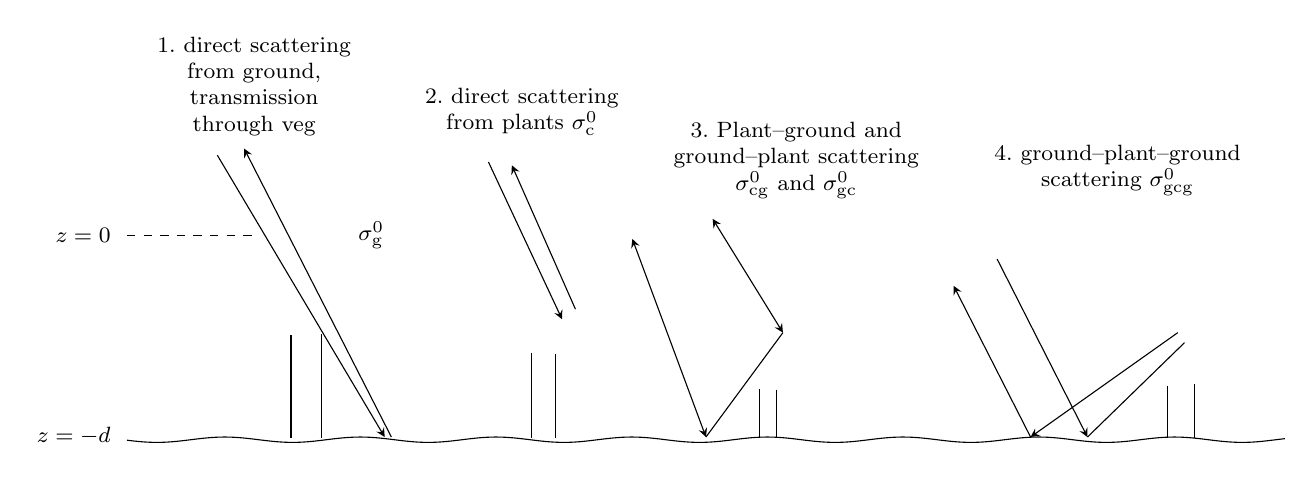
\begin{tikzpicture}[scale=0.85, >=stealth, font=\footnotesize]
		% ground and levels
		\draw plot[domain=3.1:20.4, samples=200, smooth] (\x,{0.04*sin(deg(3.1*\x))});
		\node[anchor=east] at (3.0,0.05) {$z=-d$};
		\node[anchor=east] at (3.0,3.05) {$z=0$};
		\draw[dashed] (3.1,3.05) -- (5.0,3.05);
		% trees
		\canopy{5.7}{2.35}{0.72}{0.8}
		\draw (5.55,1.56) -- (5.55,0.02); \draw (6.0,1.58) -- (6.0,0.02);
		\canopy{9.55}{2.0}{0.8}{0.72}
		\draw (9.15,1.3) -- (9.15,0.02); \draw (9.5,1.28) -- (9.5,0.02);
		\canopy{12.8}{1.5}{0.7}{0.75}
		\draw (12.55,0.76) -- (12.55,0.02); \draw (12.8,0.75) -- (12.8,0.02);
		\canopy{18.8}{1.6}{0.8}{0.8}
		\draw (18.65,0.81) -- (18.65,0.02); \draw (19.05,0.83) -- (19.05,0.02);
		% 1: direct ground
		\draw[->] (4.45,4.25) -- (6.95,0.04);
		\draw[->] (7.05,0.04) -- (4.85,4.35);
		\node[anchor=south, align=center] at (5.0,4.4) {1.~direct scattering\\from ground,\\transmission\\through veg};
		\node at (6.75,3.05) {$\sigma_\mathrm{g}^0$};
		% 2: direct volume
		\draw[->] (8.5,4.15) -- (9.6,1.8);
		\draw[->] (9.8,1.95) -- (8.85,4.1);
		\node[anchor=south, align=center] at (9.0,4.4) {2.~direct scattering\\from plants $\sigma_\mathrm{c}^0$};
		% 3: canopy-ground and ground-canopy
		\draw[<->] (10.65,3.0) -- (11.75,0.04);
		\draw (11.75,0.04) -- (12.9,1.6);
		\draw[<->] (12.9,1.6) -- (11.85,3.3);
		\node[anchor=south, align=center] at (13.1,3.45) {3.~Plant--ground and\\ground--plant scattering\\$\sigma_\mathrm{cg}^0$ and $\sigma_\mathrm{gc}^0$};
		% 4: ground-canopy-ground
		\draw[->] (16.1,2.7) -- (17.45,0.04);
		\draw (17.45,0.04) -- (18.9,1.45);
		\draw[->] (18.8,1.6) -- (16.6,0.04);
		\draw[->] (16.6,0.04) -- (15.45,2.3);
		\node[anchor=south, align=center] at (17.9,3.5) {4.~ground--plant--ground\\scattering $\sigma_\mathrm{gcg}^0$};
	\end{tikzpicture}
	\caption{Single-scattering contributions to backscatter from a vegetation canopy of height $d$ (cf.\ Ulaby and Long (2014), Fig.~11-3).}
	\label{f:paths}
\end{figure}
% NOTE: the caption is added.

\begin{itemize}
	\item Key point: top of vegetation ($z=0$) is diffuse $\Rightarrow$ no scattering; important simplification that will not be valid for all volume scattering (e.g., snow is a volume scatterer with surface scattering component).
\end{itemize}

\subsection{Extinction and transmissivity of the canopy}
\label{s:ext}

\begin{itemize}
	% NOTE: checked against U&L 2014, Eq. 11.1 (p. 462), Eq. 11.25 and delta_p = 1/kappa_e (p. 469). The handwritten
	% K_0 is written k_0 (D14). kappa_a = 2 k_0 n'' with sqrt(eps) = n' - j n'' (the effective dielectric constant of the
	% canopy); since gamma = j k_0 sqrt(eps) = k_0 n'' + j k_0 n', alpha = k_0 n'', so kappa_a = 2 alpha (power, not
	% field, attenuation), and delta_p = 1/kappa_e reduces to the Lecture 2 penetration depth 1/(2 alpha) when kappa_s = 0.
	\item To account for transmission through canopy, define $p$-polarized extinction coefficient (a.k.a.\ power attenuation factor)
	\begin{equation}
		\label{e:ke}
		\ke{p} = \kappa_\mathrm{a}^p + \kappa_\mathrm{s}^p \quad\rightarrow\quad \text{related to penetration depth} \rightarrow \delta_p = \frac{1}{\kappa_\mathrm{e}},
	\end{equation}
	\begin{itemize}
		\item[] $\kappa_\mathrm{a}^p \rightarrow$ absorption losses $\rightarrow \kappa_\mathrm{a}^p = -2k_0\,\mathrm{Im}\{\sqrt{\varepsilon}\}$ (cf.\ $\alpha$, attenuation constant, from previous lectures),
		\item[] $\kappa_\mathrm{s}^p \rightarrow$ scattering losses.
	\end{itemize}
	In general, $\ke{p}$, $\kappa_\mathrm{a}^p$, $\kappa_\mathrm{s}^p$ vary in space and time, particularly with $z$. Hereafter, assume $\ke{p}$, $\kappa_\mathrm{a}^p$, $\kappa_\mathrm{s}^p$ are uniform.
	% NOTE: checked against U&L 2014, Eqs. 11.2-11.3 (p. 463), where the exponent kappa_e^p d sec(theta_i) is called
	% the optical depth tau_p; no symbol for it is introduced here (tau is the Fresnel transmission coefficient; master
	% table F2).
	\item Now define transmissivity of canopy
	\begin{equation}
		\label{e:Ups}
		\Upsilon_p = e^{-\ke{p}d/\cos\theta_i}.
	\end{equation}
\end{itemize}

\subsection{Contribution 1: direct scattering from the ground}
% NOTE: the subsection headings "Contribution 1" ... "Contribution 4" are added; the handwriting numbers the
% contributions 1-4 as in Figure f:paths ("Let us consider each scatterer defined in the previous cartoon").

\begin{itemize}
	\item Let us consider each scatterer defined in the previous cartoon (Figure~\ref{f:paths}).
	\item Recalling the previous lecture on surface scattering, we can expect a ground-scattered component in the absence of vegetation to be $\sigma^0_{\mathrm{s},pq}(\theta_i)$. With vegetation, we expect some attenuation due to absorption and scattering in the canopy
	% NOTE: checked against U&L 2014, Eq. 11.4 (p. 463).
	\begin{equation}
		\label{e:sg}
		\Rightarrow\quad \sigma^0_{\mathrm{g},pq} = \Upsilon_p\Upsilon_q\,\sigma^0_{\mathrm{s},pq}, \qquad p,q = h \text{ or } v.
	\end{equation}
\end{itemize}

\subsection{Contribution 2: direct volume contribution}
\label{s:direct}

\begin{itemize}
	\item There are many ways to model this component.
	% NOTE: checked against U&L 2014, Eq. 11.5 and the terminology box (p. 463). U&L write sigma_v^back without the
	% hat; the handwritten hat (low-confidence reading; possibly a check accent) is kept; the handwritten subscript v
	% (volume) is dropped (instructor decision, master table D76), so sigma-hat^back_pq is written without it.
	\item By far the simplest is to treat as a ``cloud''
	\begin{equation}
		\label{e:cloud}
		\sback = N_\mathrm{v}\,\sigma^\mathrm{back}_{pq},
	\end{equation}
	where
	\begin{itemize}
		\item[] $\sback \equiv$ volume backscattering coefficient (m$^{-1}$),
		% NOTE: handwritten reads "backscattering coef of a single particle"; written "cross section" because the quantity
		% has units of m^2 (U&L 2014, p. 463: backscattering cross section of a single particle).
		\item[] $\sigma^\mathrm{back}_{pq} \equiv$ backscattering cross section of a single particle (m$^2$),
		\item[] $N_\mathrm{v} \equiv$ number of ``particles'' per unit volume (m$^{-3}$).
	\end{itemize}
	% NOTE: added "(Figure~\ref{f:cloud})"; the handwritten "visualize" introduces the sketch.
	\item Visualize (Figure~\ref{f:cloud}).
\end{itemize}

\begin{figure}[!htbp]
	\centering
	% Reproduces the handwritten sketch (page L5), element by element: the incident line labeled S_0^i (handwritten S,
	% written \mathcal{S}, D10) meeting the top ellipse (area A_0, with leader); a tube inclined at theta_i to the
	% vertical, each side solid, then dashed, then solid with a downward arrowhead; a dotted vertical below the top
	% ellipse with the arc theta_i; z = 0 (label and short dashed segments on both sides); the differential volume (top
	% ellipse labeled A = A_0/cos(theta_i) with a curved leader, bottom ellipse with dashed back half, sigma-hat_v^back
	% inside) with an arrow pointing up out of it; the dimension dz (vertical, T bars) on the left and dz/cos(theta_i)
	% (T bars) on the right; two trees and three bushes; the wavy ground z = -d.
	% NOTE: the handwritten dz/cos(theta_i) bar is vertical and as tall as the dz bar; it is drawn here parallel to the
	% tube, along the slant length that the label gives (as in U&L 2014, Fig. 11-5, "dz sec theta_i").
	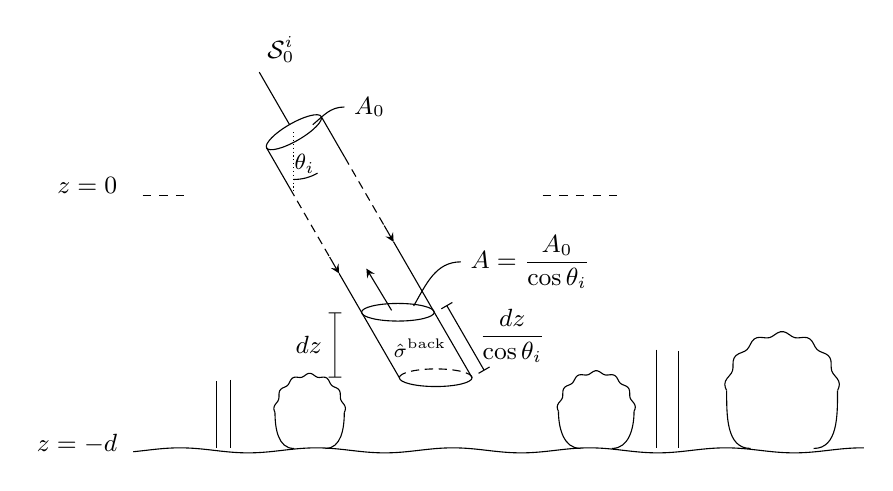
\begin{tikzpicture}[scale=0.8, >=stealth, font=\small]
		\def\ti{30}
		\pgfmathsetmacro{\s}{sin(\ti)}\pgfmathsetmacro{\c}{cos(\ti)}
		% ground, levels
		\draw plot[domain=6.3:17.9, samples=200, smooth] (\x,{0.04*sin(deg(2.9*\x))});
		\node[anchor=east] at (6.2,0.1) {$z=-d$};
		\node[anchor=east] at (6.2,4.2) {$z=0$};
		\draw[dashed] (6.45,4.05) -- (7.1,4.05);
		\draw[dashed] (12.8,4.05) -- (14.1,4.05);
		% trees and bushes
		\canopy{7.65}{2.5}{1.15}{1.4}
		\draw (7.62,1.1) -- (7.62,0.03); \draw (7.85,1.12) -- (7.85,0.03);
		\draw plot[domain=0:180, samples=60, smooth] ({9.1+0.55*(1+0.04*sin(13*\x))*cos(\x)},{0.6+0.6*(1+0.04*sin(13*\x))*sin(\x)});
		\draw (8.55,0.6) to[out=-90,in=180] (8.85,0.03); \draw (9.65,0.6) to[out=-90,in=0] (9.35,0.03);
		\canopy{15.0}{2.7}{0.98}{1.12}
		\draw (14.6,1.6) -- (14.6,0.03); \draw (14.95,1.58) -- (14.95,0.03);
		\draw plot[domain=0:180, samples=60, smooth] ({13.65+0.6*(1+0.04*sin(13*\x))*cos(\x)},{0.62+0.62*(1+0.04*sin(13*\x))*sin(\x)});
		\draw (13.05,0.62) to[out=-90,in=180] (13.4,0.03); \draw (14.25,0.62) to[out=-90,in=0] (13.9,0.03);
		\draw plot[domain=0:180, samples=60, smooth] ({16.6+0.88*(1+0.04*sin(13*\x))*cos(\x)},{0.95+0.9*(1+0.04*sin(13*\x))*sin(\x)});
		\draw (15.72,0.95) to[out=-90,in=180] (16.1,0.03); \draw (17.48,0.95) to[out=-90,in=0] (17.1,0.03);
		% tube: axis from T (top ellipse, perpendicular to the beam) along (sin, -cos); the differential volume has
		% horizontal end faces (area A, as handwritten), of half-width w/cos(theta_i)
		\def\w{0.5}
		\pgfmathsetmacro{\wh}{\w/\c}
		\coordinate (T) at (8.85,5.05);
		\coordinate (ax) at ({\s},{-\c});
		\coordinate (pr) at ({\w*\c},{\w*\s});  % half-width, perpendicular to the axis
		\coordinate (M) at ($(T)+3.3*(ax)$);   % top of the differential volume
		\coordinate (B) at ($(T)+4.5*(ax)$);   % bottom of the differential volume
		% incident line and label
		\draw ($(T)-1.1*(ax)$) -- ($(T)-0.14*(ax)$);
		\node[anchor=south west] at ($(T)-1.15*(ax)+(0.0,-0.05)$) {$\mathcal{S}_0^i$};
		% ellipses
		\draw[rotate around={\ti:(T)}] (T) ellipse ({\w} and {0.14});
		\draw (M) ellipse ({\wh} and {0.14});
		\draw (B) ++(\wh,0) arc (0:-180:{\wh} and {0.14});
		\draw[densely dashed] (B) ++(\wh,0) arc (0:180:{\wh} and {0.14});
		% tube sides: solid, dashed, solid with a downward arrowhead
		\foreach \sg in {-1,1} {
			\draw ($(T)+\sg*(pr)$) -- ($(T)+\sg*(pr)+0.75*(ax)$);
			\draw[densely dashed] ($(T)+\sg*(pr)+0.75*(ax)$) -- ($(T)+\sg*(pr)+2.0*(ax)$);
			\draw[->] ($(T)+\sg*(pr)+2.0*(ax)$) -- ($(T)+\sg*(pr)+2.3*(ax)$);
			\draw ($(T)+\sg*(pr)+2.3*(ax)$) -- ($(B)+(\sg*\wh,0)$);
		}
		% theta_i at the top ellipse
		\draw[densely dotted] (T) -- ++(0,-1.0);
		\draw ($(T)+(0,-0.75)$) arc (-90:{-90+\ti}:0.75);
		\node at ($(T)+(0.17,-0.5)$) {\footnotesize$\theta_i$};
		% A_0 label
		\draw ($(T)+(0.3,0.12)$) to[out=40,in=180] ($(T)+(0.8,0.4)$) node[right] {$A_0$};
		% upward arrow out of the element, A label
		\draw[->] ($(M)+(-0.1,0.03)$) -- ($(M)-0.8*(ax)+(-0.1,0)$);
		\draw ($(M)+(0.25,0.1)$) to[out=60,in=180] ($(M)+(1.0,0.8)$) node[right] {$A = \dfrac{A_0}{\cos\theta_i}$};
		\node at ($(M)!0.5!(B)+(0.05,-0.05)$) {\scriptsize$\hat{\sigma}^\mathrm{back}$};
		% dz (vertical) and dz/cos(theta_i) (along the tube)
		\draw[|-|] ($(M)+(-1.0,0)$) -- ($(B)+(-1.0-1.2*\s,0)$);
		\node[anchor=east] at ($(M)!0.5!(B)+(-1.05-0.6*\s,0)$) {$dz$};
		\draw[|-|] ($(M)+(\wh,0)+0.45*(pr)$) -- ($(B)+(\wh,0)+0.45*(pr)$);
		\node[anchor=west] at ($(M)!0.5!(B)+(\wh,0)+0.6*(pr)$) {$\dfrac{dz}{\cos\theta_i}$};
	\end{tikzpicture}
	\caption{Direct backscatter by a differential volume of the canopy at depth $z$: a beam of cross section $A_0$ incident at $\theta_i$ illuminates the horizontal area $A = A_0/\cos\theta_i$, and a layer of thickness $dz$ is traversed along the slant length $dz/\cos\theta_i$, so the element has geometric volume $A_0\,dz/\cos\theta_i = A\,dz$ (cf.\ Ulaby and Long (2014), Fig.~11-5).}
	\label{f:cloud}
\end{figure}
% NOTE: the caption is added. Its volume statement follows the geometry of the figure (see the NOTE after
% Eq. (e:dsig)).

\begin{itemize}
	% NOTE: handwritten S (power density) written \mathcal{S} (D10) here and below. Checked against U&L 2014, Eq. 11.6
	% (p. 464).
	\item ($q$-polarized) power density (recall Poynting vector) across area $A$ of a differential volume element within the canopy at depth $z<0$
	\begin{equation}
		\label{e:Sq}
		\mathcal{S}_q^i(z) = \mathcal{S}_0^i\cos\theta_i\,e^{\ke{q}z/\cos\theta_i} \qquad \left[\frac{\mathrm{W}}{\mathrm{m}^2}\right],
	\end{equation}
	where $\mathcal{S}_0^i \equiv$ incident power density in free space.
	% NOTE: checked against U&L 2014, Eq. 11.7 (p. 464). The handwriting labels sigma-hat with an L-shaped leader to
	% "backscattering cross section / unit volume" and the volume factor with an underbrace; both are set as
	% underbraces here.
	\item Backscattering cross section of differential volume
	\begin{equation}
		\label{e:dsig}
		d\sigma^\mathrm{back}_{pq} = \underbrace{\sback}_{\mathclap{\substack{\text{backscattering cross}\\\text{section / unit volume}}}}\qquad\quad \underbrace{\frac{A\,dz}{\cos\theta_i}}_{\substack{\text{volume of}\\\text{differential element}}} \qquad [\mathrm{m}^2].
	\end{equation}
	% NOTE: layout only: \qquad\quad added between the two factors and \mathclap dropped from the second label so the two
	% underbrace labels no longer print on top of each other; the label text is unchanged.
	% NOTE: the handwriting (following U&L 2014, Eq. 11.7, p. 464, "A sec theta_i dz") labels A dz/cos theta_i as the
	% volume of the differential element, and the equations are kept as written. Geometrically, however, the element of
	% Figure f:cloud (the part of the beam tube between the planes z and z - dz) has volume A dz = A_0 dz/cos theta_i
	% (cross section A_0 times slant length dz/cos theta_i), not A dz/cos theta_i (Monte Carlo check: A_0 = 1,
	% theta_i = 35 deg, dz = 0.5 gives 0.611, vs A dz = 0.610 and A dz/cos theta_i = 0.745). The results are unaffected
	% because S_q^i in Eq. (e:Sq) carries a factor cos theta_i (power per unit horizontal area), which cancels the extra
	% 1/cos theta_i: S_q^i dsigma = (S_q^i/cos theta_i) sigma-hat (A dz), i.e., beam power density x sigma-hat x geometric
	% volume. The explanatory sentence below is added.
	Here $A\,dz/\cos\theta_i$ is not the geometric volume of the element in Figure~\ref{f:cloud}, which is $A\,dz = A_0\,dz/\cos\theta_i$ (cross section $A_0$ times slant length $dz/\cos\theta_i$). The extra factor $1/\cos\theta_i$ is compensated by the $\cos\theta_i$ in Eq.~\eqref{e:Sq}, which gives the power per unit horizontal area rather than the power density $\mathcal{S}_q^i/\cos\theta_i$ along the beam, so the product $\mathcal{S}_q^i\,d\sigma^\mathrm{back}_{pq} = (\mathcal{S}_q^i/\cos\theta_i)\,\sback\,A\,dz$ used below is correct and the results are unaffected.
	% NOTE: the handwritten second line (partly erased) reads S_0^i A sigma-hat e^{(kappa_e^p + kappa_e^q) z/cos theta_i} dz,
	% which follows from the first line with Eqs. (e:Sq) and (e:dsig) (cos theta_i and 1/cos theta_i cancel) and is kept.
	% U&L 2014, Eq. 11.8 (p. 464), has a spurious factor 2 in this exponent, inconsistent with their own first line and
	% with Eq. 11.9; it is not propagated (python3: integrating with the factor 2 does not give Eq. 11.9).
	\item $p$-polarized power reradiated by differential volume, in the backscatter direction, after propagation from depth $z<0$ to top of canopy ($z=0$)
	\begin{align}
		dP_p^\mathrm{rer} &= \mathcal{S}_q^i(z)\,d\sigma^\mathrm{back}_{pq}\,e^{\ke{p}z/\cos\theta_i} \nonumber\\
		&= \mathcal{S}_0^i A\,\sback\,e^{(\ke{p}+\ke{q})z/\cos\theta_i}\,dz. \label{e:dP}
	\end{align}
	% NOTE: checked against U&L 2014, Eq. 11.9 (p. 464), and by python3 quadrature (kappa_e^p = 0.4, kappa_e^q = 0.7 Np/m,
	% d = 1.5 m, theta_i = 35 deg: numerical and closed forms agree to 1e-15). The handwritten third line has empty
	% braces with an arrow from the underbraced factor of the second line; the factor is written out.
	\item Integrating $dP_p^\mathrm{rer}$ over the canopy depth
	\begin{align}
		P_p^\mathrm{rer} &= \mathcal{S}_0^i A\int_{-d}^0 \sback\,e^{(\ke{p}+\ke{q})z/\cos\theta_i}\,dz \nonumber\\
		&= \left\{\frac{\mathcal{S}_0^iA\cos\theta_i\,\sback}{\ke{p}+\ke{q}}\right\}\left[1 - e^{-(\ke{p}+\ke{q})d/\cos\theta_i}\right] \nonumber\\
		&= \left\{\frac{\mathcal{S}_0^iA\cos\theta_i\,\sback}{\ke{p}+\ke{q}}\right\}\left[1 - \Upsilon_p\Upsilon_q\right]. \label{e:P}
	\end{align}
	% NOTE: handwritten r (distance to antenna) written R (D53). Checked against U&L 2014, Eq. 11.10 (p. 464) and the
	% Lecture 7 definition sigma^0 = (4 pi R^2/A)(|E_p^s|^2/|E_q^i|^2).
	\item Defining the normalized radar cross section from the canopy as
	\begin{equation}
		\label{e:sc_def}
		\sigma^0_{\mathrm{c},pq} = \frac{4\pi R^2}{A}\,\frac{\mathcal{S}_{r,p}}{\mathcal{S}_0^i}, \qquad R \equiv \text{distance to antenna},
	\end{equation}
	where
	\begin{equation*}
		\mathcal{S}_{r,p} = \frac{P_p^\mathrm{rer}}{4\pi R^2}
	\end{equation*}
	is the power density at the receiving antenna, we have
	\begin{align}
		\sigma^0_{\mathrm{c},pq} &= \frac{\sback\cos\theta_i}{\ke{p}+\ke{q}}\left(1 - \Upsilon_p\Upsilon_q\right) \nonumber\\
		&= \frac{\sback\cos\theta_i}{\ke{p}+\ke{q}}\left(1 - e^{-(\ke{p}+\ke{q})d\sec\theta_i}\right), \label{e:sc}
	\end{align}
	where $\sback$, $\ke{p}$ and $\ke{q}$ are all functions of the density and dielectric properties of the leaves and stems that make up the canopy.
\end{itemize}

\subsection{Contribution 3: canopy--ground contributions}
\label{s:cg}

\begin{itemize}
	\item Here we have reflection from ground then scattering from canopy and vice versa.
	% NOTE: checked against U&L 2014, p. 465 (quasi-specular surface).
	\item Assume the ground is a quasi-specular reflector, meaning that we only consider reflection in the specular direction but account for diffuse scattering due to surface roughness in the reflectivity.
	% NOTE: handwritten Gamma^p_coh, Gamma^p written Gamma_p^coh, Gamma_p (polarization as a subscript, as Gamma_h,
	% Gamma_v in Lecture 5 and the master table); handwritten K_0 written k_0 (D14). Checked against U&L 2014,
	% Eq. 11.11 (p. 465) and Eqs. 5.110-5.111 (p. 199), with their s = h here.
	\item Assume a very simple model
	\begin{equation}
		\label{e:Gcoh}
		\Gc{p} = \Gamma_p(\theta_i)\,e^{-4k_0^2h^2\cos^2\theta_i},
	\end{equation}
	where
	\begin{itemize}
		\item[] $\Gamma_p(\theta_i) \equiv |\rho_p|^2$, where $\rho_p \equiv$ Fresnel reflection coefficient,
		\item[] $h \equiv$ RMS height of surface roughness.
	\end{itemize}
	% NOTE: added "(Figure~\ref{f:cg})".
	\item Sketch (Figure~\ref{f:cg}).
\end{itemize}

\begin{figure}[!htbp]
	\centering
	% Reproduces the handwritten sketch (page L7), element by element: z = 0 (dashed line across both panels) and z = -d
	% (wavy ground line). Left, "ground-canopy": incident ray with a downward arrowhead partway down, the arc theta_i to a
	% short dotted vertical at its top, and the label "passes through canopy" with a curved leader; at the ground a dotted
	% normal with arcs theta_i on both sides and the label Gamma_coh; the reflected ray (no arrowhead) up to a small tilted
	% cylinder, with the ray continuing dotted inside it; a dashed horizontal line at the cylinder with the label
	% theta_i' = theta_s' = pi/2 - theta_i (written pi/2 - theta_i, D78); the scattered ray up to the top with an arrowhead at its top end, the arc
	% theta_i to a dotted vertical at the z = 0 crossing; the labels "scattered by canopy in direction of antenna" (with
	% leader), sigma-hat_v^bist and "Bistatic scattering". Right, "canopy-ground": incident ray with a downward
	% arrowhead to a tilted cylinder (sigma-hat_v^bist), the arc theta_i to a dotted vertical at the top; the scattered
	% ray down to the ground with an arrowhead near the ground; the dotted normal with arcs theta_i on both sides and
	% Gamma_coh; the reflected ray up to the top with an upward arrowhead partway up and the arc theta_i to a dotted
	% vertical at the top. Geometry drawn with theta_i = 30 deg and equal angles at the ground (as labeled).
	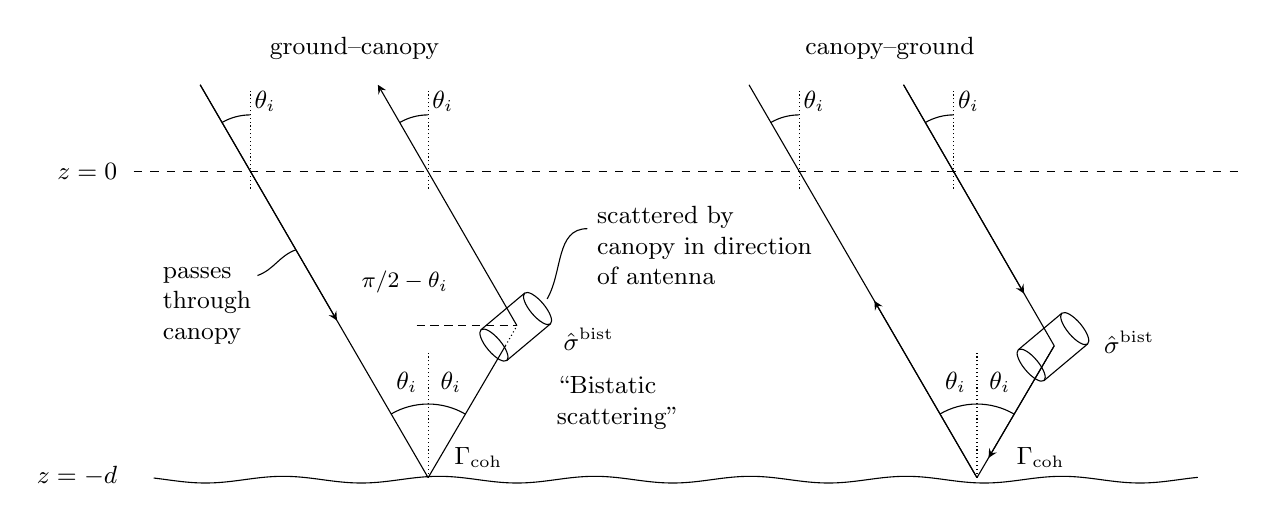
\begin{tikzpicture}[scale=0.85, >=stealth, font=\small]
		\def\ti{30}
		\pgfmathsetmacro{\t}{tan(\ti)}
		\def\Z{4.6}   % z = 0 level
		% cylinder: center #1, axis angle #2
		\newcommand{\cyl}[2]{
			\begin{scope}[shift={#1}, rotate=#2]
				\draw (-0.45,-0.3) -- (0.4,-0.3); \draw (-0.45,0.3) -- (0.4,0.3);
				\draw (-0.45,0) ellipse (0.11 and 0.3);
				\draw (0.4,0) ellipse (0.11 and 0.3);
			\end{scope}}
		% angle at a ground point #1: dotted normal, arcs theta_i on both sides
		\newcommand{\gnd}[1]{
			\draw[densely dotted] #1 -- ++(0,1.9);
			\draw ($#1+({-1.1*sin(\ti)},{1.1*cos(\ti)})$) arc ({90+\ti}:90:1.1);
			\draw ($#1+(0,1.1)$) arc (90:{90-\ti}:1.1);
			\node at ($#1+(-0.32,1.42)$) {$\theta_i$};
			\node at ($#1+(0.34,1.42)$) {$\theta_i$};}
		% angle at the top of a ray crossing z = 0 at x = #1 (ray tilted toward -x going up)
		\newcommand{\topang}[1]{
			\pgfmathsetmacro{\xa}{#1}
			\draw[densely dotted] (\xa,{\Z-0.25}) -- (\xa,{\Z+1.2});
			\draw (\xa,{\Z+0.85}) arc (90:{90+\ti}:0.85);
			\node at ({\xa+0.22},{\Z+1.05}) {$\theta_i$};}
		% levels
		\draw[dashed] (3.0,\Z) -- (19.6,\Z);
		\node[anchor=east] at (2.9,\Z) {$z=0$};
		\draw plot[domain=3.3:18.9, samples=220, smooth] (\x,{0.05*sin(deg(2.7*\x))});
		\node[anchor=east] at (2.9,0.05) {$z=-d$};
		%%% left: ground-canopy
		\node at (6.3,6.45) {ground--canopy};
		\coordinate (G) at (7.4,0.03);
		\coordinate (C) at ({7.4+2.3*\t},2.3);
		\coordinate (It) at ({7.4-5.9*\t},5.9);
		\coordinate (St) at ({7.4+2.3*\t-3.6*\t},5.9);
		\draw (It) -- (G);
		\draw[->] (It) -- ($(It)!0.6!(G)$);
		\draw (G) -- ($(C)+({-0.3*\t},-0.3)$);
		\draw[densely dotted] ($(C)+({-0.3*\t},-0.3)$) -- (C);
		\draw[->] (C) -- (St);
		\cyl{(C)}{40}
		\topang{7.4-\Z*\t}
		\topang{7.4+2.3*\t-(\Z-2.3)*\t}
		\gnd{(G)}
		\node at ($(G)+(0.75,0.3)$) {$\Gamma_\mathrm{coh}$};
		\draw[densely dashed] ($(C)+(-1.5,0)$) -- (C);
		\node[align=center, font=\footnotesize, inner sep=1pt] at (7.05,2.95) {$\pi/2 - \theta_i$};
		\node[align=left, anchor=east] at (4.9,2.6) {passes\\through\\canopy};
		\draw (4.85,3.05) to[out=20,in=200] ($(It)!0.42!(G)$);
		\node[align=left, anchor=west] at ($(C)+(1.05,1.2)$) {scattered by\\canopy in direction\\of antenna};
		\draw ($(C)+(0.45,0.4)$) to[out=60,in=180] ($(C)+(1.05,1.45)$);
		\node[anchor=west] at ($(C)+(0.55,-0.2)$) {$\hat{\sigma}^\mathrm{bist}$};
		\node[align=left, anchor=west] at ($(C)+(0.45,-1.15)$) {``Bistatic\\scattering''};
		%%% right: canopy-ground
		\node at (14.3,6.45) {canopy--ground};
		\coordinate (G2) at (15.6,0.03);
		\coordinate (C2) at ({15.6+2.0*\t},2.0);
		\coordinate (I2) at ({15.6+2.0*\t-3.9*\t},5.9);
		\coordinate (R2) at ({15.6-5.9*\t},5.9);
		\draw (I2) -- (C2);
		\draw[->] (I2) -- ($(I2)!0.8!(C2)$);
		\cyl{(C2)}{40}
		\draw (C2) -- (G2);
		\draw[->] (C2) -- ($(C2)!0.85!(G2)$);
		\draw (G2) -- (R2);
		\draw[->] (G2) -- ($(G2)!0.45!(R2)$);
		\node[anchor=west] at ($(C2)+(0.6,0.05)$) {$\hat{\sigma}^\mathrm{bist}$};
		\topang{15.6+2.0*\t-(\Z-2.0)*\t}
		\topang{15.6-\Z*\t}
		\gnd{(G2)}
		\node at ($(G2)+(0.95,0.3)$) {$\Gamma_\mathrm{coh}$};
	\end{tikzpicture}
	\caption{The two canopy--ground single-scattering contributions: ground--canopy (reflection by the ground, then bistatic scattering by the canopy toward the antenna) and canopy--ground (bistatic scattering by the canopy toward the ground, then reflection by the ground). The two follow the same path in reverse (cf.\ Ulaby and Long (2014), Fig.~11-6).}
	\label{f:cg}
\end{figure}
% NOTE: the caption is added. Gamma_coh in the figure is the handwritten label (Gamma_p^coh or Gamma_q^coh in the text).

\begin{itemize}
	% NOTE: checked against U&L 2014, Eqs. 11.12-11.13 (p. 465), and by derivation (python3 quadrature): the one-way
	% attenuation along the path (down d sec theta_i, up (d + z) sec theta_i to the element, then |z| sec theta_i back to
	% the top) totals 2 d sec theta_i for every z when p = q, and the cos theta_i of the power density cancels the
	% sec theta_i of the element volume, so sigma^0 = sigma-hat^bist d Gamma Upsilon_p Upsilon_q exactly for p = q.
	% For p != q the exponent is 2 kappa_q d + (kappa_q - kappa_p) z (depth-dependent), and the form here is U&L's
	% heuristic approximation (python3 quadrature differs slightly). The handwritten angles theta_i',
	% theta_s' (= pi/2 - theta_i) are written pi/2 - theta_i explicitly (instructor decision, master table D78). The handwritten
	% "canopy thickness" label points to d with a curved arrow from above; set as an underbrace here.
	\item Normalized radar cross sections
	\begin{itemize}
		\item[] ground--canopy:
		\begin{equation}
			\label{e:sgc}
			\sigma^0_{\mathrm{gc},pq}(\theta_i) = \sbist(\pi/2 - \theta_i)\,\underbrace{d}_{\mathclap{\text{canopy thickness}}}\,\Gc{q}\,\Upsilon_q\Upsilon_p,
		\end{equation}
		\item[] canopy--ground:
		\begin{equation}
			\label{e:scg}
			\sigma^0_{\mathrm{cg},pq}(\theta_i) = \sbist(\pi/2 - \theta_i)\,d\,\Gc{p}\,\Upsilon_p\Upsilon_q.
		\end{equation}
	\end{itemize}
	% NOTE: checked against U&L 2014, Eqs. 11.14-11.15 (p. 466).
	\item The total canopy--ground contribution
	\begin{align}
		\sigma^0_{\mathrm{cgt},pq} &= \sigma^0_{\mathrm{gc},pq} + \sigma^0_{\mathrm{cg},pq} \nonumber\\
		&= \sbist\,d\left(\Gc{p} + \Gc{q}\right)\Upsilon_p\Upsilon_q. \label{e:scgt}
	\end{align}
	\item In the case of co-polarized scattering ($p=q$), we have
	\begin{equation}
		\label{e:scgt_inc}
		\sigma^0_{\mathrm{cgt},pp} = 2\hat{\sigma}^\mathrm{bist}_{pp}\,d\,\Gc{p}\,\Upsilon_p^2.
	\end{equation}
	% NOTE: the handwritten upward arrow ("However, [arrow] not quite correct") is written "this (above)".
	\item However, this (above) is not quite correct because we added the \underline{powers} (for simplicity) rather than taking the power of the total $\mathbf{E}$ field. In other words, we undertook \underline{incoherent} addition of fields. Since ground--canopy and canopy--ground follow the same path in reverse, we should expect equivalent phase $\Rightarrow$ $\mathbf{E}$ fields add \underline{coherently}. Can correct by simply multiplying by factor of two
	\begin{equation}
		\label{e:scgt_coh}
		\Rightarrow\quad \boxed{\sigma^0_{\mathrm{cgt},pp} = 4\hat{\sigma}^\mathrm{bist}_{pp}\,d\,\Gc{p}\,\Upsilon_p^2 \qquad \text{for } p = h \text{ or } v}
	\end{equation}
\end{itemize}

\subsection{Contribution 4: ground--canopy--ground contribution}

\begin{itemize}
	\item This is very simple: 2-way transmission, 2 bounces off the ground, and backscatter from the canopy $\sigma^0_{\mathrm{c},pq}(\theta_i)$
	% NOTE: checked against U&L 2014, Eq. 11.16 (p. 466), and numerically (python3) against Eq. (e:sc).
	\begin{align}
		\Rightarrow\quad \sigma^0_{\mathrm{gcg},pq} &= \Upsilon_p\Upsilon_q\,\Gc{p}\,\Gc{q}\,\sigma^0_{\mathrm{c},pq} \nonumber\\
		&= \frac{\sback\cos\theta_i}{\ke{p}+\ke{q}}\,\Gc{p}\,\Gc{q}\left(\Upsilon_p\Upsilon_q - \Upsilon_p^2\Upsilon_q^2\right). \label{e:sgcg}
	\end{align}
\end{itemize}

% NOTE: the subsection heading is added (the handwriting has the starred bullet only).
\subsection{Putting it all together}
\label{s:total}

\begin{itemize}
	% NOTE: checked against U&L 2014, Eq. 11.17 (p. 466), where the factor c is written n; U&L also allow n = 1 for hh
	% and vv "under the incoherent addition assumption". The handwritten c is written c_add (instructor decision,
	% master table D79: c is the speed of light, and the upright subscript c denotes the canopy).
	\item[$\bigstar$] Putting it all together, the total normalized radar cross section is
	\begin{align}
		\sigma^0_{pq} &= \sigma^0_{\mathrm{g},pq} + \sigma^0_{\mathrm{c},pq} + \sigma^0_{\mathrm{cgt},pq} + \sigma^0_{\mathrm{gcg},pq} \nonumber\\
		&= \Upsilon_p\Upsilon_q\,\sigma^0_{\mathrm{s},pq}(\theta_i) + \frac{\sback\cos\theta_i}{\ke{p}+\ke{q}}\left(1 - \Upsilon_p\Upsilon_q\right)\left(1 + \Gc{p}\,\Gc{q}\,\Upsilon_p\Upsilon_q\right) \nonumber\\
		&\quad + c_\mathrm{add}\,\sbist\,d\left(\Gc{p} + \Gc{q}\right)\Upsilon_p\Upsilon_q, \label{e:total}
	\end{align}
	where
	\begin{equation*}
		c_\mathrm{add} = \begin{cases} 1 & p \ne q \quad \text{(cross-pol, incoherent addition)},\\ 2 & p = q \quad \text{(co-pol, coherent addition)}.\end{cases}
	\end{equation*}
	\item[] In general, the terms $\sigma^0_{\mathrm{s},pq}$, $\sback$, $\sbist$, $\ke{p}$ ($\Rightarrow\Upsilon_p$), $\ke{q}$ ($\Rightarrow\Upsilon_q$), $\Gc{p}$, $\Gc{q}$, and $d$ are not known a priori.
\end{itemize}

% NOTE: the subsection heading is added (in the handwriting "Simplifications" is a bullet).
\subsection{Simplifications}
\label{s:simp}

\begin{itemize}
	% NOTE: checked: d -> 0 gives Upsilon_p, Upsilon_q -> 1 and d (1 - Upsilon_p Upsilon_q) terms -> 0 (U&L 2014, p. 466).
	\item Canopy of negligible thickness:
	\begin{equation}
		\label{e:thin}
		\lim_{d\to0}\sigma^0_{pq} = \sigma^0_{\mathrm{s},pq} \qquad \text{(pure surface scattering from the ground)}.
	\end{equation}
	% NOTE: handwritten "approx" written "->" (instructor preference). Checked against U&L 2014, Eq. 11.18 (p. 466).
	\item Very thick and/or dense canopy:
	\begin{equation}
		\label{e:thick}
		\Upsilon_p,\ \Upsilon_q \rightarrow 0 \quad\Rightarrow\quad \sigma^0_{pq} \rightarrow \frac{\sback\cos\theta_i}{\ke{p}+\ke{q}}.
	\end{equation}
	% NOTE: checked against U&L 2014, Eqs. 11.19-11.21 (p. 467); kappa_s = kappa_e - kappa_a with kappa_a from
	% Eq. (e:ke). For isotropic scatterers the scattered power per unit solid angle is kappa_s/(4 pi) per unit volume,
	% so the (4 pi-normalized) volume scattering coefficient is kappa_s in every direction and for both polarizations.
	\item Isotropic scatterers:
	\begin{equation}
		\label{e:iso_s}
		\hat{\sigma}^\mathrm{back} = \hat{\sigma}^\mathrm{bist} = \kappa_\mathrm{s} = \kappa_\mathrm{e} + 2k_0\,\mathrm{Im}\{\sqrt{\varepsilon}\}
		\qquad \left(\text{note } \kappa_\mathrm{e} = \kappa_\mathrm{s} + \kappa_\mathrm{a},\ \kappa_\mathrm{a} = -2k_0\,\mathrm{Im}\{\sqrt{\varepsilon}\}\right)
	\end{equation}
	and $\Upsilon_p = \Upsilon_q$
	% NOTE: handwritten reads Upsilon^2 sigma^0_pp(theta_i) for the first term; corrected to Upsilon^2
	% sigma^0_s,pp(theta_i) (bare-ground scattering coefficient) because this term is the ground contribution
	% Upsilon_p Upsilon_q sigma^0_s,pq of Eq. (e:total) (same page), as in U&L 2014, Eq. 11.20 (p. 467); without the s
	% the symbol is the total sigma^0_pp of the left-hand side. Also added the definitions of Upsilon and Gamma^coh.
	% The algebra from Eq. (e:total) with c_add = 2 was checked numerically (python3).
	\begin{equation}
		\label{e:iso}
		\Rightarrow\quad \sigma^0_{pp} = \Upsilon^2\sigma^0_{\mathrm{s},pp}(\theta_i) + \frac{\kappa_\mathrm{s}}{\kappa_\mathrm{e}}\,\frac{\cos\theta_i}{2}\left(1 - \Upsilon^2\right)\left(1 + (\Gamma^\mathrm{coh})^2\Upsilon^2\right) + 4\kappa_\mathrm{s}\,d\,\Gamma^\mathrm{coh}\,\Upsilon^2,
	\end{equation}
	where $\Upsilon \equiv \Upsilon_p$ and $\Gamma^\mathrm{coh} \equiv \Gc{p}$.
	% NOTE: checked against U&L 2014, Eqs. 11.22-11.23 (p. 467); the algebra from Eq. (e:total) was checked
	% numerically (python3). Correction of scope: U&L state sigma_v^back = sigma_v^bist = (3/2) kappa_s "for hh and vv
	% polarizations and for the incident and scattered directions shown in Fig. 11-6". The backscatter value holds for
	% both polarizations, but in the specular bistatic geometry of Figure f:cg the wave is turned through the scattering
	% angle 2 theta_i, and the dipole pattern of a Rayleigh particle gives (3/2) kappa_s for hh (E perpendicular to the
	% scattering plane) but (3/2) kappa_s cos^2(2 theta_i) for vv (E in the scattering plane). Evidence: Liou (2002),
	% Eq. 3.3.7a,b (p. 89): I_r independent of the scattering angle Theta, I_l proportional to cos^2 Theta; U&L's own
	% Rayleigh phase matrix, Eq. 11.55a (p. 475), psi_11 = (3 kappa_s/8 pi)(sin theta_s sin theta_i + cos theta_s
	% cos theta_i)^2 in the plane of incidence, which with the incident direction at pi - theta_i (from below, after
	% reflection) and theta_s = theta_i gives cos^2(2 theta_i), and gives 1 in exact backscatter (Eq. 11.56); python3
	% check with explicit dipole vectors (vv factor 0.883, 0.25, 0, 0.25 at theta_i = 10, 30, 45, 60 deg). The
	% handwritten equations are therefore kept and scoped to hh, and the vv form of the last term is added.
	\item Rayleigh scatterers (spheres with radius $\ll\lambda$):
	\begin{equation}
		\label{e:ray_s}
		\hat{\sigma}^\mathrm{back} = \hat{\sigma}^\mathrm{bist} = \frac{3}{2}\kappa_\mathrm{s}
		\qquad (\text{bistatic value: } hh;\ \text{see below for } vv)
	\end{equation}
	\begin{equation}
		\label{e:ray}
		\Rightarrow\quad \sigma^0_{pp}(\theta_i) = \Upsilon^2\sigma^0_{\mathrm{s},pp} + \frac{3}{4}\,\frac{\kappa_\mathrm{s}}{\kappa_\mathrm{e}}\cos\theta_i\left(1 - \Upsilon^2\right)\left(1 + (\Gamma^\mathrm{coh})^2\Upsilon^2\right) + 3c_\mathrm{add}\,\kappa_\mathrm{s}\,d\,\Gamma^\mathrm{coh}\,\Upsilon^2.
	\end{equation}
	(For $vv$, the dipole scattering pattern reduces the bistatic value in the specular geometry of Figure~\ref{f:cg}, where the scattering angle is $2\theta_i$, to $\hat{\sigma}^\mathrm{bist} = \frac{3}{2}\kappa_\mathrm{s}\cos^2 2\theta_i$, so the last term of Eq.~\eqref{e:ray} becomes $3c_\mathrm{add}\,\kappa_\mathrm{s}\,d\,\Gamma^\mathrm{coh}\cos^2(2\theta_i)\,\Upsilon^2$; the backscatter value $\frac{3}{2}\kappa_\mathrm{s}$ holds for both polarizations.)
	\item General considerations for models of $\hat{\sigma}^\mathrm{back}$ and $\hat{\sigma}^\mathrm{bist}$:
	\begin{itemize}
		\item density of scatterers;
		\item size of scatterers relative to EM wavelength;
		\item if size $\gtrsim\lambda$, shape and orientation of scatterers.
	\end{itemize}
\end{itemize}

%%%%%%%%%%%%%%%%%%%%%%%%%%%%%%%%%%%%%
\section{Heuristic model of scattering from a snow layer of depth $d$}
\label{s:snow}

\begin{itemize}
	\item The volume scattering will be identical to the vegetation model, but now we must account for reflection and transmission at the air--snow interface.
	% NOTE: handwritten T_p, T_q (transmissivities) written \mathbb{T}_p, \mathbb{T}_q (D19; master table \mathbb{T}_h,
	% \mathbb{T}_v, L5). Checked against U&L 2014, Eq. 11.24 (p. 468), where the transmissivities are evaluated at
	% theta_i and, because of refraction, theta_i is replaced by the angle of propagation in the snow (U&L theta_i';
	% written theta_t, the master-table angle of refraction) in Upsilon and in the rest of the vegetation model; inside
	% the snow the ground terms are those of the snow-ground interface (U&L: "sigma^0_sg is the snow-ground
	% backscattering coefficient", p. 468), and the ground reflectivity is set by the snow-soil dielectric contrast.
	% These parentheticals are added.
	\item Straightforward extension of previous model
	\begin{equation}
		\label{e:snow}
		\sigma^0_{pq}(\theta_i) = \mathbb{T}_p\,\mathbb{T}_q\left(\sigma^0_{pq}\big|_\mathrm{veg}\right) + \sigma^0_{\mathrm{as},pq},
	\end{equation}
	where
	\begin{itemize}
		\item[] $\mathbb{T}_p$ and $\mathbb{T}_q$ are transmissivity of air--snow interface (at $\theta_i$),
		\item[] $\sigma^0_{pq}|_\mathrm{veg}$ is the model derived previously for vegetation scattering (Eq.~\eqref{e:total}, evaluated at the angle of refraction $\theta_t$ into the snow, with $\sigma^0_{\mathrm{s},pq}$ and $\Gamma_p^\mathrm{coh}$ those of the snow--ground interface),
		\item[] $\sigma^0_{\mathrm{as},pq}$ is surface scattering from air--snow interface.
	\end{itemize}
\end{itemize}

%%%%%%%%%%%%%%%%%%%%%%%%%%%%%%%%%%%%%
\section{Summary}
\label{s:summary}

\begin{itemize}
	\item Volume scattering involves scattering from dielectric discontinuities within a volume.
	\item Reflectivity of a volume is function of
	\begin{itemize}
		\item dielectric discontinuities within the volume;
		\item density of dielectric heterogeneities.
	\end{itemize}
	\item Directionality of scattering
	\begin{itemize}
		\item roughness of boundary;
		\item average dielectric constant of media;
		\item size of inclusions.
	\end{itemize}
	\item Modeling of volume scattering depends on
	\begin{itemize}
		\item size distribution of scatterers (relative to $\lambda$);
		\item orientation of scatterers;
		\item shape of scatterers;
		\item dielectric contrast.
	\end{itemize}
	\item Multiple scattering contributions from volume. E.g., vegetation
	\begin{itemize}
		\item direct ground with 2-way transmission through volume;
		\item direct canopy contribution;
		\item ground--canopy and canopy--ground;
		\item ground--canopy--ground.
	\end{itemize}
	\item For volumes with nondiffuse surface, must consider transmission through and scattering from interface.
\end{itemize}

%%%%%%%%%%%%%%%%%%%%%%%%%%%%%%%%%%%%%
% Symbols follow the master table in ../variables_master.tex; see it for flagged dual usages.
\clearpage
\section*{Variables}

Units are SI. Values are given for universal constants; ``typical'' values are representative, not definitive.

{\small
\renewcommand{\arraystretch}{1.25}
\begin{longtable}{>{$}l<{$} >{\raggedright\arraybackslash}p{0.40\textwidth} >{\raggedright\arraybackslash}p{0.13\textwidth} >{\raggedright\arraybackslash}p{0.22\textwidth}}
\hline
\textrm{Symbol} & Description & Units & Value \\
\hline
\endfirsthead
\hline
\textrm{Symbol} & Description & Units & Value \\
\hline
\endhead
\hline
\endfoot
\multicolumn{4}{l}{\emph{Geometry and general}} \\
\lambda & EM wavelength & m & -- \\
k_0 & free-space wavenumber, $2\pi/\lambda_0$ & rad/m & -- \\
\lambda_0 & free-space wavelength & m & -- \\
\theta_i & angle of incidence & rad & -- \\
\theta_t & angle of refraction (into the snow) & rad & -- \\
z & vertical coordinate ($z=0$ top of the canopy, $z=-d$ ground) & m & -- \\
d & canopy (or snow-layer) thickness & m & -- \\
p,\ q & receive and transmit polarizations & -- & $h$ or $v$ \\
R & distance to the antenna & m & -- \\
A_0 & cross-sectional area of the incident beam & m$^2$ & -- \\
A & horizontal area illuminated at depth $z$ & m$^2$ & $A_0/\cos\theta_i$ \\
\multicolumn{4}{l}{\emph{Extinction and transmission}} \\
\kappa_\mathrm{e}^p & extinction coefficient ($p$ polarization) & Np/m & $\kappa_\mathrm{a}^p + \kappa_\mathrm{s}^p$ \\
\kappa_\mathrm{a}^p & absorption coefficient & Np/m & $-2k_0\,\mathrm{Im}\{\sqrt{\varepsilon}\}$ \\
\kappa_\mathrm{s}^p & scattering coefficient & Np/m & -- \\
\varepsilon & (effective) dielectric constant of the canopy medium & dimensionless & -- \\
\alpha & attenuation constant (Lecture 2) & Np/m & $\kappa_\mathrm{a} = 2\alpha$ \\
\delta_p & penetration depth & m & $1/\kappa_\mathrm{e}$ \\
\Upsilon_p & one-way transmissivity of the canopy & dimensionless & $e^{-\kappa_\mathrm{e}^pd/\cos\theta_i}$ \\
\mathbb{T}_p & transmissivity of the air--snow interface & dimensionless & $0$--$1$ \\
\multicolumn{4}{l}{\emph{Scattering}} \\
\sigma^0_{pq} & total normalized radar cross section & dimensionless & -- \\
\sigma^0_{\mathrm{s},pq} & backscattering coefficient of the bare ground surface & dimensionless & -- \\
\sigma^0_{\mathrm{g},pq},\ \sigma^0_{\mathrm{c},pq} & direct ground and direct canopy contributions & dimensionless & -- \\
\sigma^0_{\mathrm{gc},pq},\ \sigma^0_{\mathrm{cg},pq} & ground--canopy and canopy--ground contributions & dimensionless & -- \\
\sigma^0_{\mathrm{cgt},pq} & total canopy--ground contribution & dimensionless & $\sigma^0_{\mathrm{gc},pq} + \sigma^0_{\mathrm{cg},pq}$ \\
\sigma^0_{\mathrm{gcg},pq} & ground--canopy--ground contribution & dimensionless & -- \\
\sigma^0_{\mathrm{as},pq} & backscattering coefficient of the air--snow interface & dimensionless & -- \\
\hat{\sigma}^\mathrm{back}_{pq} & volume backscattering coefficient & m$^{-1}$ & $N_\mathrm{v}\sigma^\mathrm{back}_{pq}$ \\
\hat{\sigma}^\mathrm{bist}_{pq} & volume bistatic scattering coefficient & m$^{-1}$ & -- \\
\sigma^\mathrm{back}_{pq} & backscattering cross section of a single particle & m$^2$ & -- \\
N_\mathrm{v} & number of particles per unit volume & m$^{-3}$ & -- \\
d\sigma^\mathrm{back}_{pq} & backscattering cross section of a differential volume & m$^2$ & -- \\
c_\mathrm{add} & coherent-addition factor & dimensionless & 1 ($p\ne q$), 2 ($p=q$) \\
\multicolumn{4}{l}{\emph{Power}} \\
\mathcal{S}_0^i & incident power density in free space & W/m$^2$ & -- \\
\mathcal{S}_q^i(z) & $q$-polarized power density across $A$ at depth $z$ & W/m$^2$ & -- \\
\mathcal{S}_{r,p} & $p$-polarized power density at the receiving antenna & W/m$^2$ & $P_p^\mathrm{rer}/(4\pi R^2)$ \\
P_p^\mathrm{rer} & $p$-polarized power reradiated by the canopy & W & -- \\
\multicolumn{4}{l}{\emph{Ground reflection}} \\
\Gamma_p & Fresnel reflectivity of the ground, $|\rho_p|^2$ & dimensionless & $0$--$1$ \\
\Gamma_p^\mathrm{coh} & coherent reflectivity of the rough ground & dimensionless & $\Gamma_p e^{-4k_0^2h^2\cos^2\theta_i}$ \\
\Upsilon, \Gamma^\mathrm{coh} & shorthand for $\Upsilon_p$, $\Gamma_p^\mathrm{coh}$ in co-polarized forms (Eqs.~\ref{e:iso}--\ref{e:ray}) & dimensionless & -- \\
\rho_p & Fresnel reflection coefficient & dimensionless & -- \\
h & RMS height of the ground roughness & m & -- \\
\end{longtable}
}

\end{document}
